\clearpage
\section{Hasil Eksperimen dan Analisis}
\subsection{Rancangan Eksperimen}
Seluruh model dievaluasi pada 5.475 baris validasi yang sama, hasil pembagian berstrata dengan \texttt{seed=42}. Model dilatih pada 21.856 baris latih yang telah dibersihkan. Untuk konfigurasi terpilih, validasi silang lima lipatan dijalankan pada seluruh \path{train.csv}, dengan pipeline di-\textit{fit} ulang pada setiap lipatan. Metrik berbasis label memakai ambang 0,5, kecuali pada analisis \textit{cost-sensitive}.

Metrik utama pemilihan konfigurasi adalah akurasi, sesuai metrik yang diasumsikan untuk leaderboard Kaggle. F1 kelas batal dan ROC-AUC dilaporkan sebagai pelengkap, karena akurasi saja dapat menyamarkan kemampuan model mendeteksi kelas minoritas. Setiap akurasi dibandingkan dengan baseline kelas mayoritas sebesar 0,6723.

Angka pada bab ini berasal dari eksekusi ulang notebook pengumpulan dari sel pertama hingga terakhir dengan versi pustaka pada \path{requirements.txt}. Eksekusi ulang menghasilkan CSV KNN, DTL, \textit{logistic regression}, dan \textit{Naive Bayes} yang identik dengan berkas pada \path{output/}. CSV SVM polinomial berbeda pada 9 dari 6.844 baris, yang diduga berasal dari perbedaan pembulatan aritmetika titik mengambang pada SMO. Selisih kecil juga terlihat pada metrik DTL dibanding catatan di notebook (akurasi 0,8451 berbanding 0,8449), tetapi CSV DTL tetap identik.

\subsection{Hasil per Algoritma}
\subsubsection{\textit{k-Nearest Neighbors}}\label{sec:hasil-knn}
Tabel~\ref{tab:knn-grid} memperlihatkan pengaruh $k$ dan pembobotan pada jarak Euclidean. Pembobotan jarak selalu lebih baik daripada pembobotan seragam pada setiap $k$, dengan selisih akurasi 1,2 hingga 3,0 poin persentase. Pembobotan seragam mencapai akurasi tertinggi pada $k=5$ lalu menurun, sedangkan pembobotan jarak membaik hingga $k=15$ dan tetap stabil sesudahnya. Hal ini terjadi karena bobot $1/d$ meredam pengaruh tetangga jauh yang ikut terhitung ketika $k$ membesar.

\begin{table}[htbp]
    \centering
    \small
    \begin{tabular}{@{}r l r r r r r@{}}
        \toprule
        $k$ & Bobot & Akurasi & Presisi & \textit{Recall} & F1 & ROC-AUC \\
        \midrule
        5 & \textit{uniform} & 0,8188 & 0,7416 & 0,6862 & 0,7128 & 0,8743 \\
        5 & \textit{distance} & 0,8312 & 0,7544 & 0,7191 & 0,7363 & 0,8878 \\
        15 & \textit{uniform} & 0,8179 & 0,7589 & 0,6511 & 0,7009 & 0,8827 \\
        15 & \textit{distance} & \textbf{0,8429} & 0,7876 & 0,7129 & \textbf{0,7484} & 0,9047 \\
        25 & \textit{uniform} & 0,8126 & 0,7623 & 0,6221 & 0,6851 & 0,8779 \\
        25 & \textit{distance} & 0,8413 & 0,7937 & 0,6968 & 0,7421 & \textbf{0,9055} \\
        41 & \textit{uniform} & 0,8119 & 0,7656 & 0,6137 & 0,6813 & 0,8722 \\
        41 & \textit{distance} & 0,8413 & 0,8013 & 0,6856 & 0,7390 & 0,9049 \\
        \bottomrule
    \end{tabular}
    \caption{Pengaruh $k$ dan pembobotan pada KNN (jarak Euclidean, data validasi).}
    \label{tab:knn-grid}
\end{table}

Dengan $k=15$ dan pembobotan jarak, jarak Manhattan memberi akurasi 0,8489, lebih tinggi daripada Euclidean (0,8429) dan Minkowski $p=3$ (0,8378). Jarak Manhattan tidak mengkuadratkan selisih, sehingga satu fitur dengan selisih besar tidak mendominasi jarak. Sifat ini menguntungkan pada data campuran yang memuat banyak kolom \textit{one-hot}. Konfigurasi $k=15$, Manhattan, bobot jarak dipilih untuk \textit{submission}.

\begin{table}[htbp]
    \centering
    \small
    \begin{tabular}{@{}l r r r r r@{}}
        \toprule
        Variasi \textit{preprocessing} & Akurasi & Presisi & \textit{Recall} & F1 & ROC-AUC \\
        \midrule
        Pipeline baku & 0,8489 & 0,7998 & 0,7191 & 0,7573 & 0,9106 \\
        20 fitur \textit{mutual information} teratas & 0,8515 & 0,8056 & 0,7207 & 0,7608 & 0,9099 \\
        PCA 95\% ragam (25 komponen) & 0,8462 & 0,7920 & 0,7196 & 0,7541 & 0,9053 \\
        \textit{Random oversampling} & 0,8201 & 0,6820 & 0,8450 & 0,7548 & 0,9063 \\
        \bottomrule
    \end{tabular}
    \caption{Pengaruh seleksi fitur, PCA, dan \textit{oversampling} pada KNN terpilih.}
    \label{tab:knn-variasi}
\end{table}

Tabel~\ref{tab:knn-variasi} menunjukkan bahwa seleksi 20 fitur menaikkan akurasi sebesar 0,26 poin persentase, karena kolom yang hampir tidak informatif berhenti menambah derau pada jarak. Kenaikan tersebut kecil dan hanya teramati pada satu pembagian, sehingga pipeline baku tetap dipakai untuk menjaga \textit{submission} yang sudah ada tetap \textit{reproducible}. PCA sedikit menurunkan kinerja karena proyeksi linear mencampur fitur penting dengan fitur lemah. \textit{Oversampling} menaikkan \textit{recall} dari 0,7191 menjadi 0,8450, tetapi presisi dan akurasi turun tajam. Hasil ini wajar, karena salinan sampel minoritas memperbanyak tetangga positif di sekitar setiap titik kueri sehingga model lebih sering menebak batal.

Validasi silang lima lipatan untuk konfigurasi terpilih menghasilkan rata-rata akurasi 0,8429, F1 0,7484, dan ROC-AUC 0,9049. Akurasi per lipatan berkisar 0,8409 hingga 0,8453. Rentang yang sempit ini menunjukkan bahwa kinerja KNN stabil terhadap perubahan pembagian data, dan skor pada pembagian validasi utama (0,8489) sedikit di atas rata-rata.

\subsubsection{\textit{Decision Tree Learning}}
Pohon C4.5 tanpa pemangkasan tumbuh hingga 4.634 simpul dengan kedalaman maksimum 20. Pada data validasi, pohon ini memperoleh akurasi 0,8451, presisi 0,7877, \textit{recall} 0,7219, F1 0,7533, dan ROC-AUC 0,8980. Kinerjanya hampir setara dengan KNN terbaik, padahal pohon bekerja langsung pada kategori asli dan nilai hilang tanpa imputasi.

Gambar~\ref{fig:dtl-top3} menampilkan tiga simpul pemisah teratas. Akar memilih \texttt{days\_before\_arrival} dengan ambang 154,5 hari. Pada pemesanan yang lebih dekat dengan kedatangan, peluang batal turun menjadi 23,7\%, dan tamu dengan riwayat pemesanan selesai (\texttt{prior\_completed\_bookings} $>0{,}5$) hampir tidak pernah batal (0,4\%). Pada pemesanan lebih dari 154,5 hari, peluang batal naik menjadi 70,9\% dan mencapai 89,9\% untuk tarif di atas sekitar Rp1,69 juta. Struktur ini konsisten dengan temuan \textit{data understanding} bahwa \texttt{days\_before\_arrival} adalah fitur paling informatif.

\begin{figure}[htbp]
    \centering
    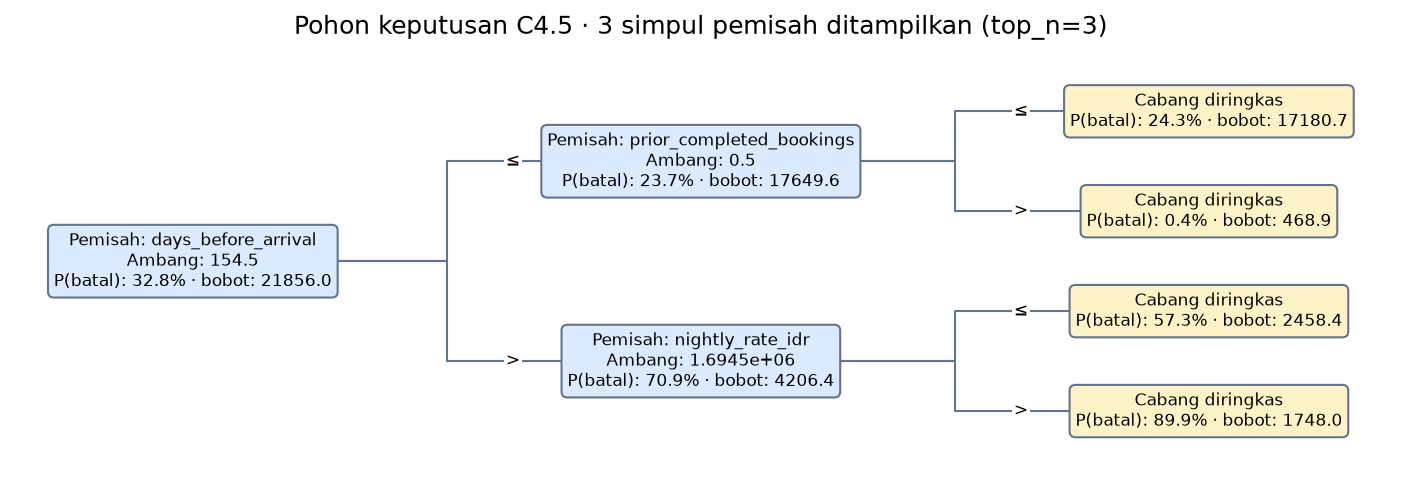
\includegraphics[width=\textwidth]{output/decision_tree_top_3.png}
    \caption{Visualisasi pohon C4.5 dengan \texttt{top\_n=3}. Simpul kuning masih memiliki keturunan yang diringkas.}
    \label{fig:dtl-top3}
\end{figure}

Parameter \texttt{top\_n} membatasi jumlah simpul pemisah yang dibuka secara melebar dari akar. Simpul yang masih memiliki anak setelah batas tercapai ditandai ``Cabang diringkas''. Gambar~\ref{fig:dtl-top7} menampilkan \texttt{top\_n=7} dengan aturan yang lebih rinci.

\begin{figure}[htbp]
    \centering
    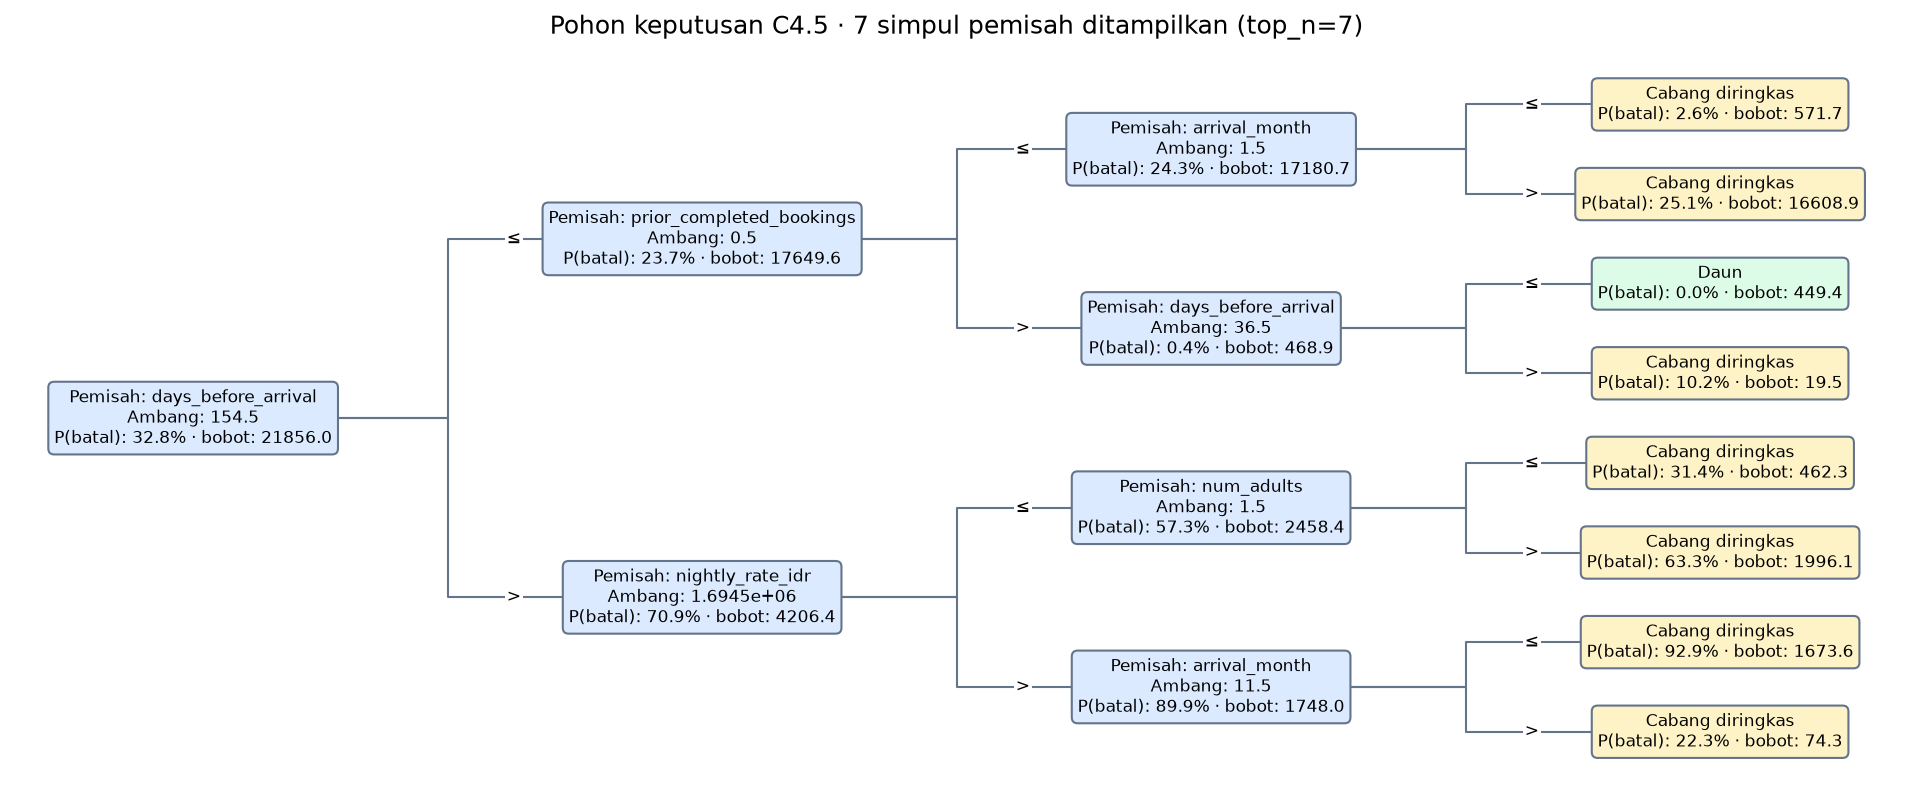
\includegraphics[width=\textwidth]{output/decision_tree_top_7.png}
    \caption{Visualisasi pohon C4.5 dengan \texttt{top\_n=7}.}
    \label{fig:dtl-top7}
\end{figure}

\subsubsection{\textit{Logistic Regression}}
Tabel~\ref{tab:lr} merangkum ketiga regularisasi dengan $\alpha=0{,}01$. Ketiganya konvergen dan menghasilkan akurasi yang sangat berdekatan, yaitu 0,7956 hingga 0,7980. Perbedaan utamanya terletak pada jumlah bobot yang bernilai nol. L1 menghasilkan 22 dari 34 bobot tepat nol, Elastic Net 19, dan L2 tidak ada. Hasil ini sesuai teori pada Gambar~\ref{fig:teori-lr}. Model L1 hanya memakai 12 fitur tetapi akurasinya turun kurang dari 0,25 poin persentase, sehingga sebagian besar fitur tidak menambah daya pisah linear. Elastic Net dipilih untuk \textit{submission} karena akurasinya tertinggi.

\begin{table}[htbp]
    \centering
    \small
    \begin{tabular}{@{}l r r r r r r r@{}}
        \toprule
        Penalti & \textit{Epoch} & Bobot nol & Akurasi & Presisi & \textit{Recall} & F1 & ROC-AUC \\
        \midrule
        L1 & 1.752 & 22 & 0,7956 & 0,7433 & 0,5747 & 0,6482 & 0,8507 \\
        L2 & 1.322 & 0 & 0,7965 & 0,7374 & 0,5886 & 0,6547 & 0,8538 \\
        Elastic Net & 1.142 & 19 & \textbf{0,7980} & 0,7436 & 0,5853 & \textbf{0,6550} & 0,8527 \\
        \bottomrule
    \end{tabular}
    \caption{Hasil \textit{logistic regression} dengan tiga regularisasi.}
    \label{tab:lr}
\end{table}

\textit{Logistic regression} memiliki akurasi terendah kedua di antara kelima model, dengan \textit{recall} hanya sekitar 0,58. Model ini hanya mampu membentuk batas keputusan linear, sedangkan hubungan fitur dengan pembatalan bersifat tidak linear. Contohnya, pengaruh \texttt{arrival\_month} bersifat musiman, dan pohon menunjukkan bahwa efek tarif bergantung pada \texttt{days\_before\_arrival}. Interaksi seperti ini tidak dapat ditangkap oleh satu hyperplane tanpa rekayasa fitur tambahan.

\subsubsection{\textit{Support Vector Machine}}
Tabel~\ref{tab:svm} menyajikan hasil ketiga kernel pada subsampel 4.000 baris serta satu eksperimen Gaussian pada subsampel 12.000 baris. Kernel polinomial memberi akurasi tertinggi pada 4.000 baris (0,8113) dan dipilih untuk \textit{submission}. Kernel linear mencapai batas 100.000 iterasi SMO sebelum konvergen dan memperoleh hasil yang mirip dengan \textit{logistic regression}, karena keduanya sama-sama pemisah linear.

\begin{table}[htbp]
    \centering
    \footnotesize
    \setlength{\tabcolsep}{4pt}
    \begin{tabular}{@{}l r r r c r r r r r@{}}
        \toprule
        Kernel & $n$ & $C$ & SV & Konvergen & Iterasi & Akurasi & \textit{Recall} & F1 & ROC-AUC \\
        \midrule
        Linear & 4.000 & 1 & 1.882 & tidak & 100.000 & 0,7934 & 0,5847 & 0,6497 & 0,8510 \\
        Polinomial ($d=3$) & 4.000 & 1 & 1.791 & ya & 60.733 & 0,8113 & 0,6081 & 0,6787 & 0,8660 \\
        Gaussian & 4.000 & 10 & 1.842 & ya & 28.242 & 0,8100 & 0,5998 & 0,6742 & 0,8597 \\
        Gaussian ($\gamma=0{,}03$) & 12.000 & 10 & 5.208 & ya & 107.164 & \textbf{0,8268} & \textbf{0,6394} & \textbf{0,7076} & \textbf{0,8784} \\
        \bottomrule
    \end{tabular}
    \caption{Hasil SVM per kernel. SV menyatakan jumlah \textit{support vector}.}
    \label{tab:svm}
\end{table}

Memperbesar subsampel dari 4.000 menjadi 12.000 baris menaikkan akurasi Gaussian dari 0,8100 menjadi 0,8268 dan ROC-AUC dari 0,8597 menjadi 0,8784, dengan waktu pelatihan sekitar 32 detik. Hasil ini menunjukkan bahwa batas utama SVM pada tugas ini adalah jumlah data latih yang dapat dimuat, bukan pilihan kernel. Jumlah \textit{support vector} sekitar 43--47\% dari data latih pada semua konfigurasi, yang menandakan banyaknya sampel di dalam margin akibat tumpang tindih kelas yang besar.

\subsubsection{\textit{Naive Bayes}}\label{sec:hasil-nb}
\textit{Naive Bayes} dengan fitur asli, $\alpha=1$, dan 20 interval memperoleh akurasi 0,7784, F1 0,6452, dan ROC-AUC 0,8364 pada data validasi. Tabel~\ref{tab:nb-cv} memperlihatkan hasil validasi silang. Penambahan fitur turunan menaikkan \textit{recall} tetapi menurunkan akurasi dan F1. Penyebabnya adalah pelanggaran asumsi kebebasan bersyarat. Fitur \texttt{total\_nights} merupakan jumlah dari \texttt{weekend\_nights} dan \texttt{weekday\_nights}, sehingga informasi yang sama dihitung dua kali dan peluang posterior menjadi terlalu yakin.

\begin{table}[htbp]
    \centering
    \small
    \begin{tabular}{@{}l r r r r r@{}}
        \toprule
        Konfigurasi (rata-rata 5 lipatan) & Akurasi & Presisi & \textit{Recall} & F1 & ROC-AUC \\
        \midrule
        Fitur asli, 20 interval & 0,7812 & 0,6871 & 0,6099 & 0,6462 & 0,8347 \\
        Fitur asli + turunan, 20 interval & 0,7677 & 0,6489 & 0,6342 & 0,6415 & 0,8224 \\
        \midrule
        Fitur asli, 5 interval & 0,7814 & 0,6930 & 0,5978 & 0,6419 & 0,8227 \\
        Fitur asli, 10 interval & 0,7790 & 0,6846 & 0,6037 & 0,6416 & 0,8255 \\
        Fitur asli, 30 interval & 0,7816 & 0,6877 & 0,6110 & 0,6470 & 0,8354 \\
        Fitur asli, 40 interval & 0,7821 & 0,6883 & 0,6122 & 0,6480 & 0,8355 \\
        \bottomrule
    \end{tabular}
    \caption{Validasi silang \textit{Naive Bayes} untuk pilihan fitur dan jumlah interval.}
    \label{tab:nb-cv}
\end{table}

Jumlah interval berpengaruh kecil. Empat puluh interval memberi F1 tertinggi (0,6480), hanya 0,0018 di atas 20 interval, sehingga 20 interval dipertahankan agar CSV yang sudah dikumpulkan tetap \textit{reproducible}. Gambar~\ref{fig:nb-graph} menampilkan graf struktur model. Tebal panah menyatakan \textit{mutual information} antara fitur dan kelas yang dihitung dari tabel peluang model. \texttt{days\_before\_arrival} menyumbang 0,1506 bit atau sekitar 41\% dari total, dan lima fitur teratas menyumbang sekitar 82\%. \texttt{prior\_completed\_bookings} bernilai nol karena hanya 2,2\% barisnya positif, sehingga seluruh batas kuantil runtuh menjadi satu interval. Kelemahan diskretisasi kuantil ini menjelaskan sebagian selisih kinerja \textit{Naive Bayes} terhadap pohon, yang justru memakai fitur tersebut pada simpul kedua.

\begin{figure}[htbp]
    \centering
    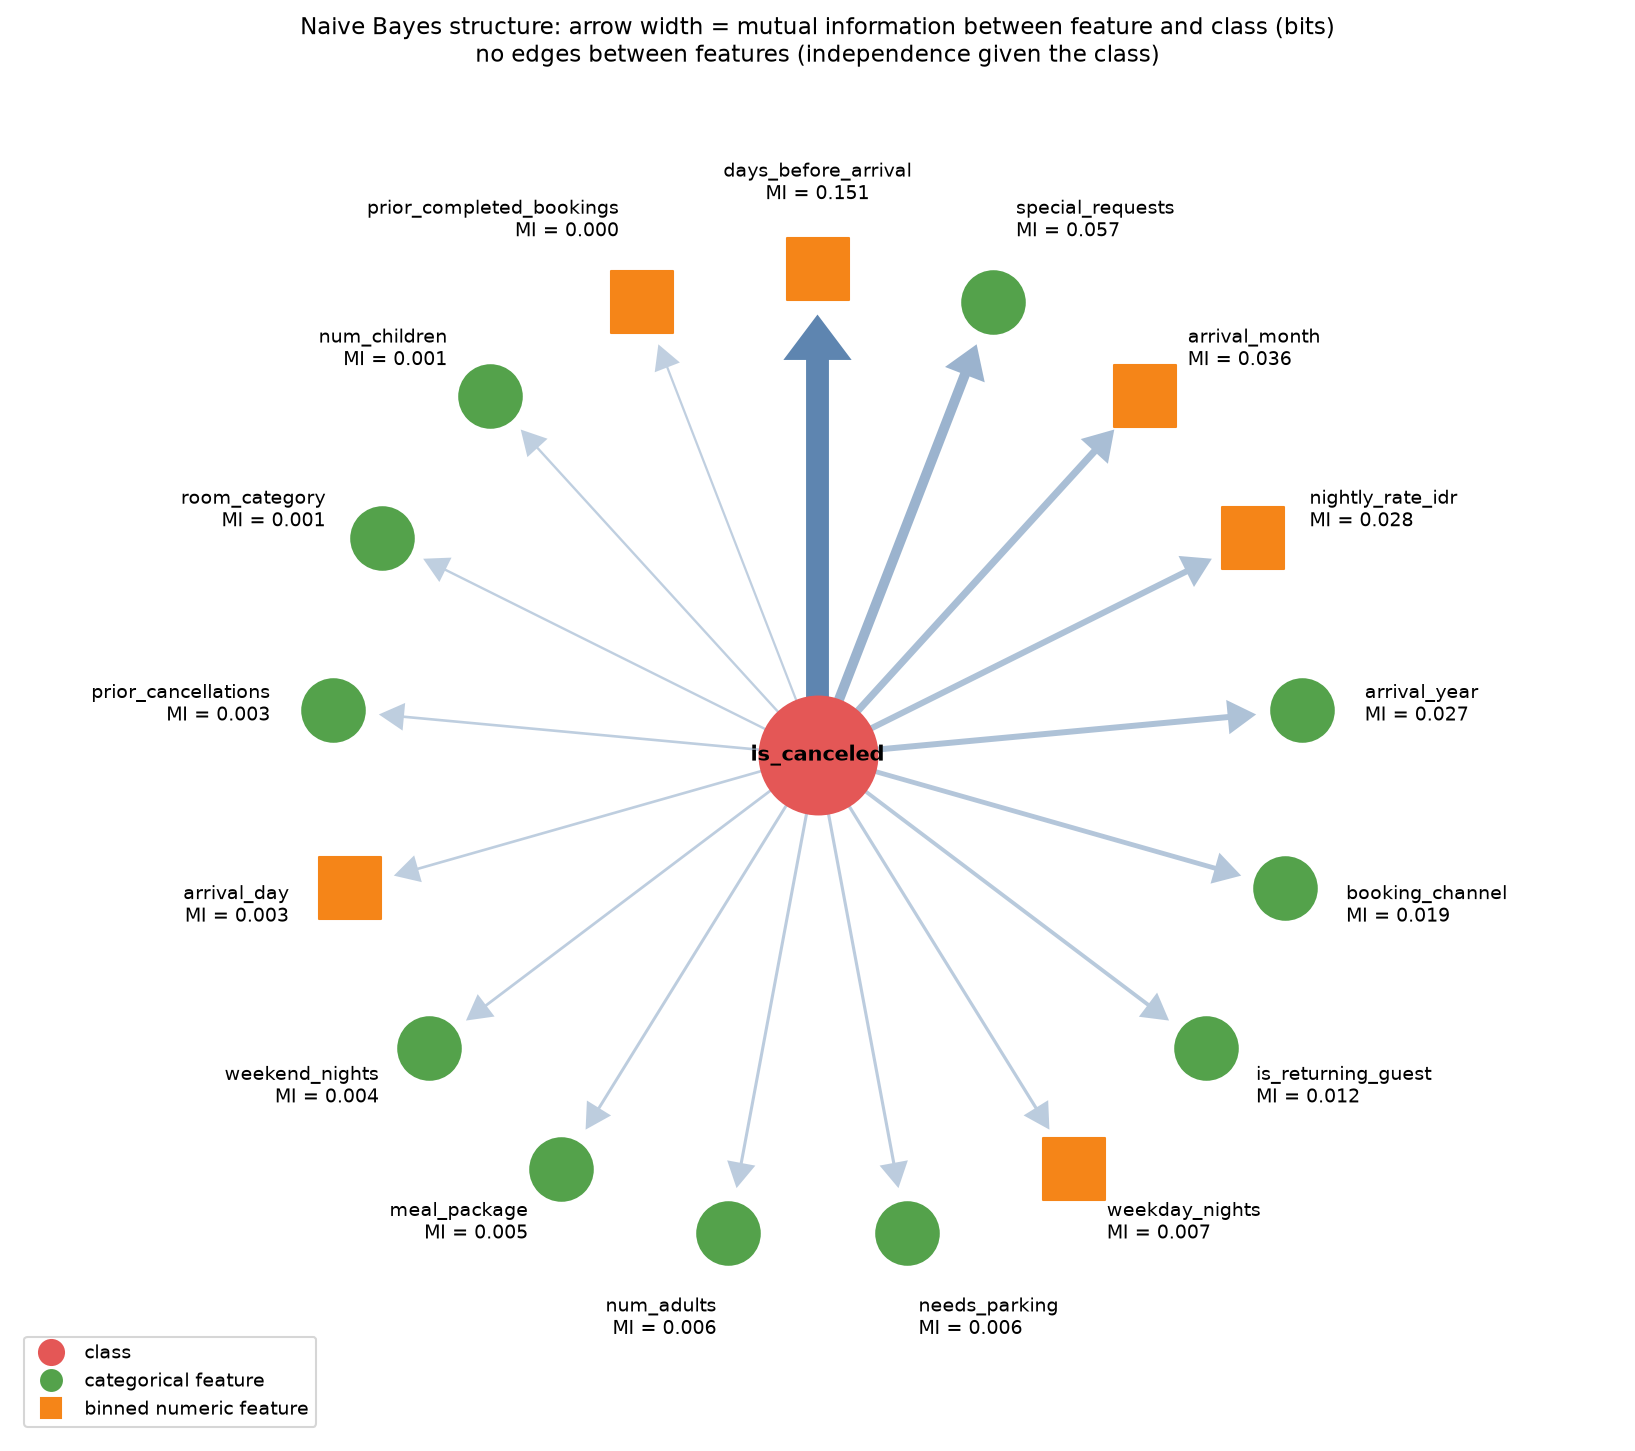
\includegraphics[width=0.78\textwidth]{output/naive_bayes_graph.png}
    \caption{Graf struktur \textit{Naive Bayes}. Lingkaran hijau adalah fitur kategorikal dan persegi jingga adalah fitur numerik yang didiskretisasi.}
    \label{fig:nb-graph}
\end{figure}

\subsection{Perbandingan Antarmodel}
Tabel~\ref{tab:ringkasan} merangkum seluruh konfigurasi pada data validasi yang sama. Semua model melampaui baseline 0,6723 dengan selisih lebar.

\begin{table}[htbp]
    \centering
    \footnotesize
    \setlength{\tabcolsep}{4pt}
    \begin{tabular}{@{}l c r r r r r@{}}
        \toprule
        Model & \textit{Submission} & Akurasi & Presisi & \textit{Recall} & F1 & ROC-AUC \\
        \midrule
        KNN ($k=15$, Manhattan, \textit{distance}) & ya & \textbf{0,8489} & \textbf{0,7998} & 0,7191 & \textbf{0,7573} & \textbf{0,9106} \\
        DTL C4.5 & ya & 0,8451 & 0,7877 & \textbf{0,7219} & 0,7533 & 0,8980 \\
        \textit{Logistic regression} L1 & & 0,7956 & 0,7433 & 0,5747 & 0,6482 & 0,8507 \\
        \textit{Logistic regression} L2 & & 0,7965 & 0,7374 & 0,5886 & 0,6547 & 0,8538 \\
        \textit{Logistic regression} Elastic Net & ya & 0,7980 & 0,7436 & 0,5853 & 0,6550 & 0,8527 \\
        SVM linear (4.000) & & 0,7934 & 0,7310 & 0,5847 & 0,6497 & 0,8510 \\
        SVM polinomial (4.000) & ya & 0,8113 & 0,7678 & 0,6081 & 0,6787 & 0,8660 \\
        SVM Gaussian (4.000) & & 0,8100 & 0,7697 & 0,5998 & 0,6742 & 0,8597 \\
        SVM Gaussian (12.000) & & 0,8268 & 0,7921 & 0,6394 & 0,7076 & 0,8784 \\
        \textit{Naive Bayes} & ya & 0,7784 & 0,6788 & 0,6148 & 0,6452 & 0,8364 \\
        \midrule
        Baseline kelas mayoritas & & 0,6723 & -- & 0 & 0 & 0,5000 \\
        \bottomrule
    \end{tabular}
    \caption{Ringkasan kinerja seluruh konfigurasi pada data validasi.}
    \label{tab:ringkasan}
\end{table}

Model terbagi ke dalam tiga kelompok yang jelas. KNN dan DTL berada di urutan teratas dengan akurasi sekitar 0,845--0,849 dan \textit{recall} di atas 0,72. Keduanya adalah model nonparametrik yang mampu membentuk batas keputusan lokal dan menangkap interaksi antarfitur. SVM berkernel menempati posisi tengah. Kemampuannya membentuk batas tidak linear dibatasi oleh subsampel. \textit{Logistic regression}, SVM linear, dan \textit{Naive Bayes} berada di urutan bawah. Dua yang pertama dibatasi oleh bentuk linear, sedangkan \textit{Naive Bayes} dibatasi oleh asumsi kebebasan bersyarat yang dilanggar oleh fitur yang saling berkaitan.

Kesalahan yang paling membedakan model adalah \textit{false negative}. Semua model memiliki tingkat FP di bawah 0,15, tetapi tingkat FN berkisar dari 0,28 untuk KNN dan DTL hingga 0,43 untuk \textit{logistic regression} L1. Model linear cenderung memprediksi kelas mayoritas pada kasus yang ambigu, sehingga banyak pembatalan tidak terdeteksi.

\subsection{Perbandingan dengan \textit{scikit-learn}}
Tabel~\ref{tab:sklearn} membandingkan setiap implementasi \textit{from scratch} dengan pembandingnya pada data latih dan validasi yang sama.

\begin{table}[htbp]
    \centering
    \small
    \setlength{\tabcolsep}{4pt}
    \begin{tabularx}{\textwidth}{@{}l l r r r r X@{}}
        \toprule
        Model & Implementasi & Akurasi & F1 & ROC-AUC & & Keterangan \\
        \midrule
        KNN & \textit{scratch} & 0,8489 & 0,7573 & 0,9106 & & \multirow{2}{=}{Identik pada empat desimal.} \\
            & \texttt{KNeighborsClassifier} & 0,8489 & 0,7573 & 0,9106 & & \\
        DTL & C4.5 \textit{scratch} & 0,8451 & 0,7533 & 0,8980 & & \multirow{2}{=}{Algoritma \textit{split} berbeda.} \\
            & \texttt{DecisionTreeClassifier} & 0,8446 & 0,7582 & 0,9016 & & \\
        LR L1 & \textit{scratch} & 0,7956 & 0,6482 & 0,8507 & & \multirow{2}{=}{Selisih koefisien maks. 0,0201.} \\
            & \texttt{LogisticRegression} & 0,7962 & 0,6493 & 0,8506 & & \\
        LR L2 & \textit{scratch} & 0,7965 & 0,6547 & 0,8538 & & \multirow{2}{=}{Selisih koefisien maks. 0,0100.} \\
            & \texttt{LogisticRegression} & 0,7969 & 0,6553 & 0,8538 & & \\
        LR EN & \textit{scratch} & 0,7980 & 0,6550 & 0,8527 & & \multirow{2}{=}{Selisih koefisien maks. 0,0142.} \\
            & \texttt{LogisticRegression} & 0,7980 & 0,6550 & 0,8527 & & \\
        SVM RBF & \textit{scratch} (12.000) & 0,8268 & 0,7076 & 0,8784 & & \multirow{2}{=}{ROC-AUC sama, kalibrasi berbeda.} \\
            & \texttt{SVC} (12.000) & 0,8263 & 0,7062 & 0,8784 & & \\
        NB & \textit{scratch} & 0,7784 & 0,6452 & 0,8364 & & \multirow{2}{=}{Beda perlakuan nilai hilang.} \\
            & \texttt{CategoricalNB} & 0,7790 & 0,6460 & 0,8344 & & \\
        \bottomrule
    \end{tabularx}
    \caption{Perbandingan implementasi \textit{from scratch} dengan \textit{scikit-learn}.}
    \label{tab:sklearn}
\end{table}

Implementasi KNN menghasilkan metrik yang identik dengan \texttt{KNeighborsClassifier} pada parameter yang sama, sehingga perhitungan jarak, pemilihan tetangga, dan pembobotan dapat dianggap benar. Implementasi \textit{logistic regression} menghasilkan metrik yang hampir sama dengan \textit{solver} SAGA setelah skala penalti disesuaikan. Selisih koefisien terbesar 0,0201 berasal dari kriteria berhenti yang berbeda, bukan dari fungsi tujuan.

Untuk SVM, pembanding \texttt{SVC} dilatih pada subsampel yang sama. Tanda fungsi keputusan kedua implementasi cocok pada 99,89\% (linear) hingga 100\% (polinomial dan Gaussian) baris validasi, dan jumlah \textit{support vector} hanya berbeda paling banyak dua. Pada eksperimen 12.000 baris, ROC-AUC keduanya sama hingga empat desimal. Selisih akurasi muncul karena \texttt{SVC} mengalibrasi peluang dengan validasi silang internal, sedangkan implementasi kelompok memakai baris di luar subsampel.

Untuk \textit{Naive Bayes}, uji ekuivalensi dengan kode kategori dan interval yang disamakan menghasilkan selisih peluang maksimum $6{,}5\times10^{-15}$ dan prediksi 100\% sama pada baris tanpa nilai hilang. Perbedaan kecil pada alur lengkap berasal dari prapemrosesan. Model kelompok melewati fitur yang hilang, sedangkan pembanding mengodekannya sebagai kategori tersendiri. Pada validasi silang, rata-rata akurasi keduanya 0,7812 dan 0,7810.

Implementasi DTL tidak dapat dibandingkan secara identik. Pembanding \texttt{DecisionTreeClassifier} hanya membentuk pohon biner, tidak mendukung atribut kategorikal secara langsung, dan memakai \textit{cost-complexity pruning} alih-alih aturan C4.5. Dengan \texttt{criterion='entropy'} dan \texttt{ccp\_alpha=0.001} sebagai padanan C4.5, akurasi keduanya berdekatan (0,8451 dan 0,8446). Pembanding memiliki \textit{recall} dan ROC-AUC sedikit lebih tinggi karena pemangkasan menghasilkan peluang daun yang lebih halus.

\subsection{Analisis Kesalahan}
Tabel~\ref{tab:error} memperlihatkan \textit{confusion matrix} kelima konfigurasi pengumpulan. KNN dan DTL memiliki jumlah FN paling sedikit, sedangkan \textit{Naive Bayes} memiliki FP paling banyak (522) karena peluangnya kurang terkalibrasi.

\begin{table}[htbp]
    \centering
    \small
    \begin{tabular}{@{}l r r r r r r@{}}
        \toprule
        Model & TN & FP & FN & TP & Tingkat FP & Tingkat FN \\
        \midrule
        KNN & 3.358 & 323 & 504 & 1.290 & 0,0877 & 0,2809 \\
        DTL C4.5 & 3.332 & 349 & 499 & 1.295 & 0,0948 & 0,2781 \\
        LR Elastic Net & 3.319 & 362 & 744 & 1.050 & 0,0983 & 0,4147 \\
        SVM polinomial & 3.351 & 330 & 703 & 1.091 & 0,0896 & 0,3919 \\
        SVM Gaussian (12.000) & 3.380 & 301 & 647 & 1.147 & 0,0818 & 0,3606 \\
        \textit{Naive Bayes} & 3.159 & 522 & 691 & 1.103 & 0,1418 & 0,3852 \\
        \bottomrule
    \end{tabular}
    \caption{\textit{Confusion matrix} pada data validasi (ambang 0,5).}
    \label{tab:error}
\end{table}

Analisis per kelompok fitur pada DTL menunjukkan bahwa kesalahan sangat bergantung pada \texttt{days\_before\_arrival}. Pada pemesanan paling lama tujuh hari sebelum kedatangan, model melewatkan 42 dari 69 pembatalan (tingkat FN 60,9\%). Pembatalan pada rentang ini jarang terjadi, sehingga daun pohon didominasi kelas tidak batal. Sebaliknya, pada rentang lebih dari 90 hari, model hanya melewatkan 151 dari 1.072 pembatalan (14,1\%), tetapi tingkat FP-nya tertinggi, yaitu 16,3\%. Pola serupa terlihat pada kanal Corporate, dengan tingkat FN 51,6\% karena pembatalan pada kanal ini jarang terjadi. Dengan kata lain, model mengandalkan rasio pembatalan dasar setiap kelompok, sehingga pembatalan pada kelompok yang jarang batal sulit dideteksi.

\subsection{\textit{Cost-Sensitive Classification}}
Pada persoalan ini, FP berarti model memprediksi batal padahal tamu datang. Jika kamar tersebut dijual ulang, hotel mengalami \textit{overbooking}, sehingga FP dianggap dua kali lebih mahal daripada FN. Penanganan berubah pada tiga hal. Pertama, aturan keputusan memakai ambang sekitar 2/3 sesuai Persamaan~\ref{eq:cost-threshold}, bukan 0,5. Kedua, kriteria pemilihan ambang adalah biaya total $2\,FP+FN$, bukan akurasi atau F1. Ketiga, ukuran yang dilaporkan adalah biaya bersama presisi dan \textit{recall}. Model tidak perlu dilatih ulang.

\begin{lstlisting}[emph={threshold_curve,fit_threshold_proba},caption={Pencarian ambang dengan biaya minimum (\texttt{src/cost\_sensitive.py})},label={lst:cost}]
def threshold_curve(proba, y, cost_fp=2.0, cost_fn=1.0):
    values, inverse = np.unique(proba, return_inverse=True)
    positives = np.bincount(inverse, weights=y, minlength=len(values))
    negatives = np.bincount(inverse, weights=1 - y, minlength=len(values))
    thresholds = np.concatenate([[values[0]], (values[:-1] + values[1:]) / 2,
                                 [np.nextafter(values[-1], np.inf)]])
    missed = np.concatenate([[0.0], np.cumsum(positives)])                 # FN
    false_alarms = negatives.sum() - np.concatenate([[0.0], np.cumsum(negatives)])  # FP
    return thresholds, cost_fp * false_alarms + cost_fn * missed
\end{lstlisting}

Fungsi \texttt{threshold\_curve} menghitung biaya untuk setiap ambang kandidat sekaligus dengan jumlah kumulatif, lalu \texttt{fit\_threshold\_proba} memilih ambang berbiaya minimum. Bila beberapa ambang memiliki biaya sama, dipilih yang paling dekat dengan 2/3. Karena ambang dicari pada data validasi yang sama dengan data penilaian, kelompok juga menghitung estimasi \textit{cross-fit}, yaitu ambang dicari pada separuh data validasi lalu dinilai pada separuh lainnya, dan sebaliknya.

\begin{table}[htbp]
    \centering
    \small
    \setlength{\tabcolsep}{3.5pt}
    \resizebox{\textwidth}{!}{%
    \begin{tabular}{@{}l r r r r r r r r r@{}}
        \toprule
        & & \multicolumn{3}{c}{Ambang 0,5} & \multicolumn{3}{c}{Ambang hasil pencarian} & & \\
        \cmidrule(lr){3-5}\cmidrule(lr){6-8}
        Model & $\tau^*$ & FP & FN & Biaya & FP & FN & Biaya & Biaya $\tau=2/3$ & Hemat \textit{cross-fit} \\
        \midrule
        KNN & 0,660 & 323 & 504 & 1.150 & 134 & 765 & \textbf{1.033} & 1.038 & 8,70\% \\
        DTL C4.5 & 0,667 & 349 & 499 & 1.197 & 225 & 685 & 1.135 & 1.137 & 3,43\% \\
        LR Elastic Net & 0,603 & 362 & 744 & 1.468 & 192 & 985 & 1.369 & 1.414 & 5,79\% \\
        SVM polinomial & 0,606 & 330 & 703 & 1.363 & 201 & 859 & 1.261 & 1.275 & 6,53\% \\
        SVM Gaussian (12.000) & 0,737 & 301 & 647 & 1.249 & 120 & 922 & 1.162 & 1.169 & 5,76\% \\
        \textit{Naive Bayes} & 0,669 & 522 & 691 & 1.735 & 194 & 975 & 1.363 & 1.367 & 20,75\% \\
        \bottomrule
    \end{tabular}}
    \caption{Biaya total $2\,FP+FN$ sebelum dan sesudah penyesuaian ambang pada data validasi.}
    \label{tab:cost}
\end{table}

Tabel~\ref{tab:cost} menunjukkan bahwa ambang 0,5 selalu lebih mahal daripada ambang hasil pencarian. Penghematan biaya pada data validasi berkisar 5,2\% (DTL) hingga 21,4\% (\textit{Naive Bayes}), dan estimasi \textit{cross-fit} tetap positif untuk semua model, yaitu 3,4\% hingga 20,8\%. Pada KNN, FP turun dari 323 menjadi 134 (58,5\%), sedangkan FN naik dari 504 menjadi 765. Presisi naik dari 0,7998 menjadi 0,8848, sedangkan \textit{recall} turun dari 0,7191 menjadi 0,5736. Model menjadi lebih berhati-hati menandai pemesanan sebagai batal, sehingga risiko \textit{overbooking} berkurang dengan konsekuensi lebih banyak pembatalan yang tidak terdeteksi.

Ambang hasil pencarian mendekati 2/3 pada delapan dari sepuluh konfigurasi, dan aturan teoretis $\tau=2/3$ hampir sama baiknya. Selisih biaya terbesar hanya 45 pada \textit{logistic regression} Elastic Net. \textit{Naive Bayes} paling diuntungkan karena peluangnya cenderung ekstrem akibat asumsi kebebasan. Dengan ambang 0,5 biayanya tertinggi, tetapi setelah penyesuaian biayanya setara dengan \textit{logistic regression}. Gambar~\ref{fig:cost} memperlihatkan bahwa setiap kurva biaya membentuk lembah datar di sekitar ambang 0,6--0,75, sedangkan ambang 0,5 masih berada di sisi yang menurun. Kurva KNN dan DTL berbentuk tangga karena peluang keduanya hanya mengambil sedikit nilai berbeda.

\begin{figure}[htbp]
    \centering
    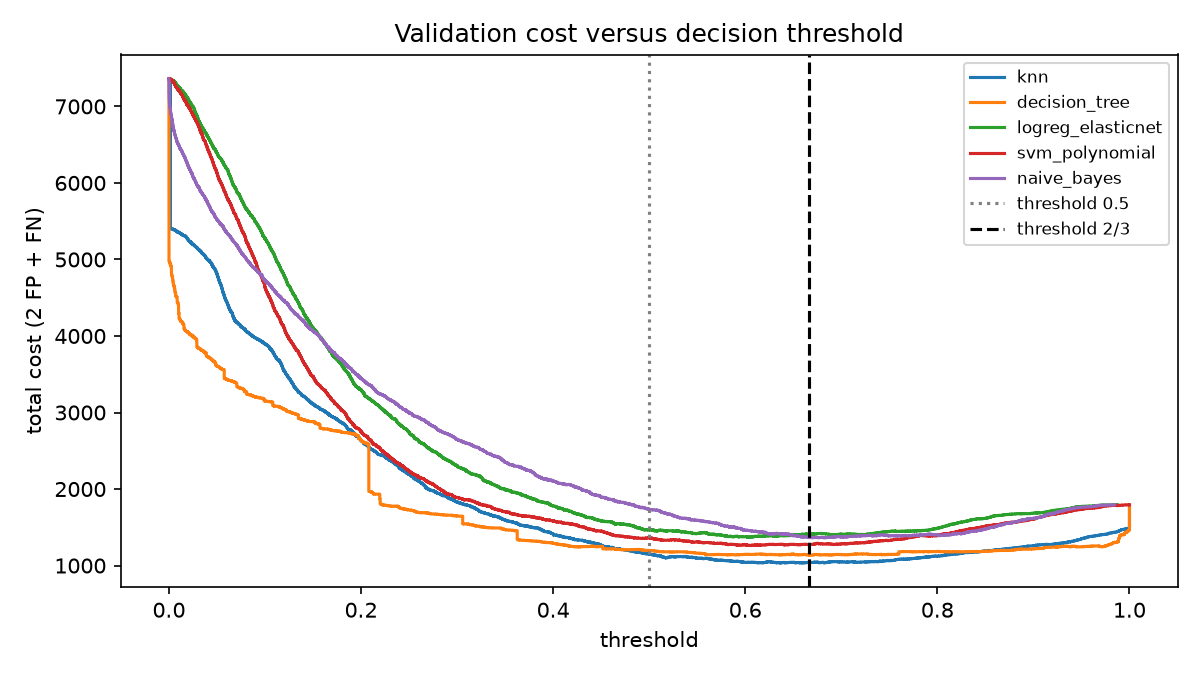
\includegraphics[width=0.85\textwidth]{output/cost_vs_threshold.png}
    \caption{Biaya total validasi terhadap ambang keputusan untuk lima konfigurasi pengumpulan.}
    \label{fig:cost}
\end{figure}

\subsection{Visualisasi Model}
\subsubsection{Video Kontur \textit{Log-Loss}}
Agar \textit{loss} hanya bergantung pada dua parameter, model dilatih pada satu fitur, yaitu \texttt{days\_before\_arrival} terstandardisasi, tanpa regularisasi, dengan laju belajar 0,05 selama 300 \textit{epoch}. Metode \texttt{plot\_loss\_contour\_video} menghitung \textit{log-loss} pada kisi $(\theta_0,\theta_1)$, menggambar konturnya, lalu menganimasikan lintasan parameter dari \texttt{history\_}. Video disimpan sebagai \path{output/lr_loss_contour.mp4}. Gambar~\ref{fig:lr-video} menampilkan bingkai terakhir. Lintasan bergerak dari $(0,0)$ dengan \textit{log-loss} 0,6931 menuju $(\theta_0,\theta_1)=(-0{,}7457;\,0{,}9001)$ dengan \textit{log-loss} 0,5400. Lintasan tegak lurus terhadap kontur, sesuai sifat \textit{gradient descent}, dan langkahnya memendek ketika mendekati minimum karena gradien mengecil.

\begin{figure}[htbp]
    \centering
    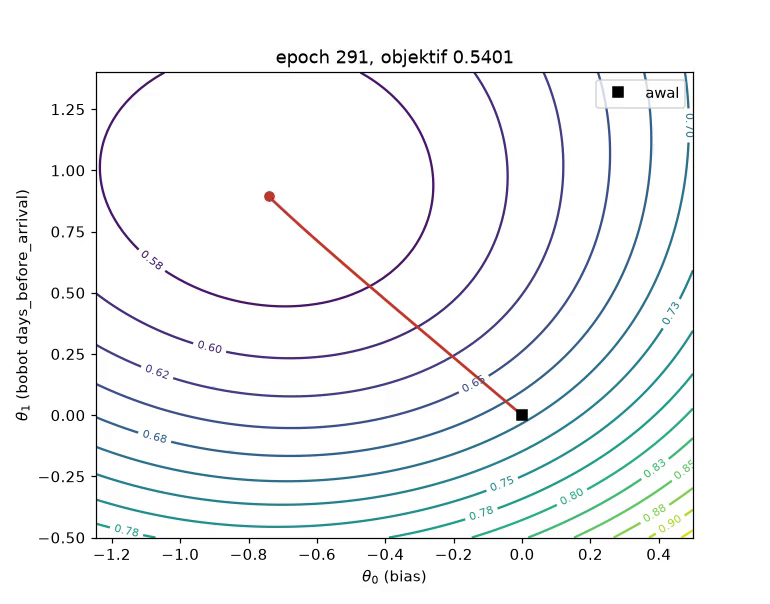
\includegraphics[width=0.62\textwidth]{figures/lr_loss_contour_last.png}
    \caption{Bingkai terakhir video kontur \textit{log-loss} dan lintasan parameter.}
    \label{fig:lr-video}
\end{figure}

\subsubsection{Bidang Pemisah SVM}
Visualisasi memakai fitur \texttt{days\_before\_arrival} dan \texttt{nightly\_rate\_idr} hasil \textit{preprocessing}. Setiap kernel dilatih dengan $C=1$ pada subsampel berstrata 2.000 baris. Garis utuh menyatakan batas keputusan $f(\mathbf{x})=0$, garis putus-putus menyatakan margin $f(\mathbf{x})=\pm1$, dan lingkaran hitam menandai \textit{support vector}. Kernel linear menghasilkan garis lurus dengan 1.158 \textit{support vector}, polinomial menghasilkan kurva dengan 1.089, dan Gaussian menghasilkan daerah tertutup yang lebih lokal dengan 1.063 \textit{support vector}. Pada ketiga gambar, kedua kelas sangat bertumpang tindih di bidang dua fitur ini, sehingga lebih dari separuh sampel menjadi \textit{support vector}.

\begin{figure}[htbp]
    \centering
    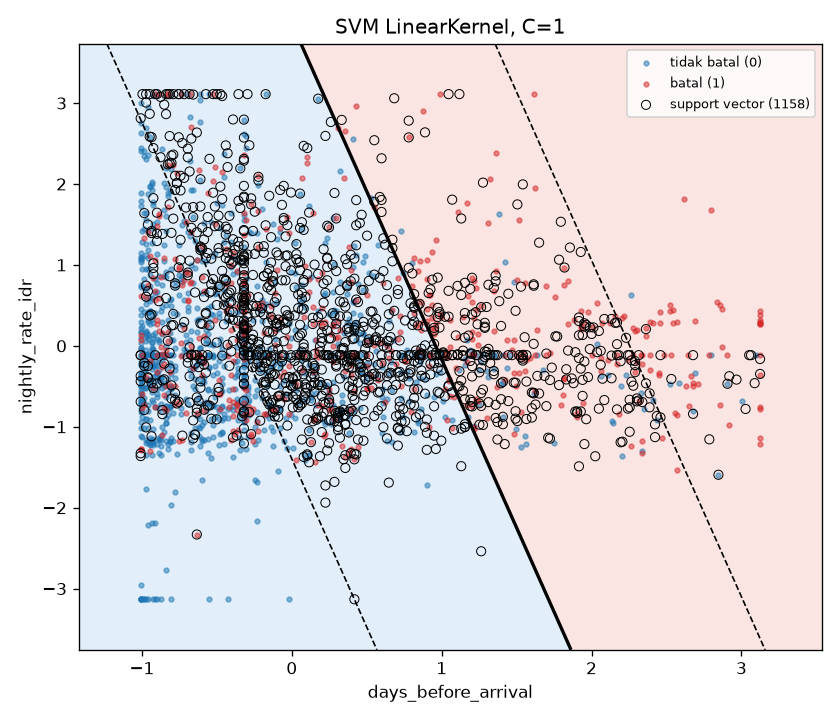
\includegraphics[width=0.32\textwidth]{output/svm_boundary_linear.png}\hfill
    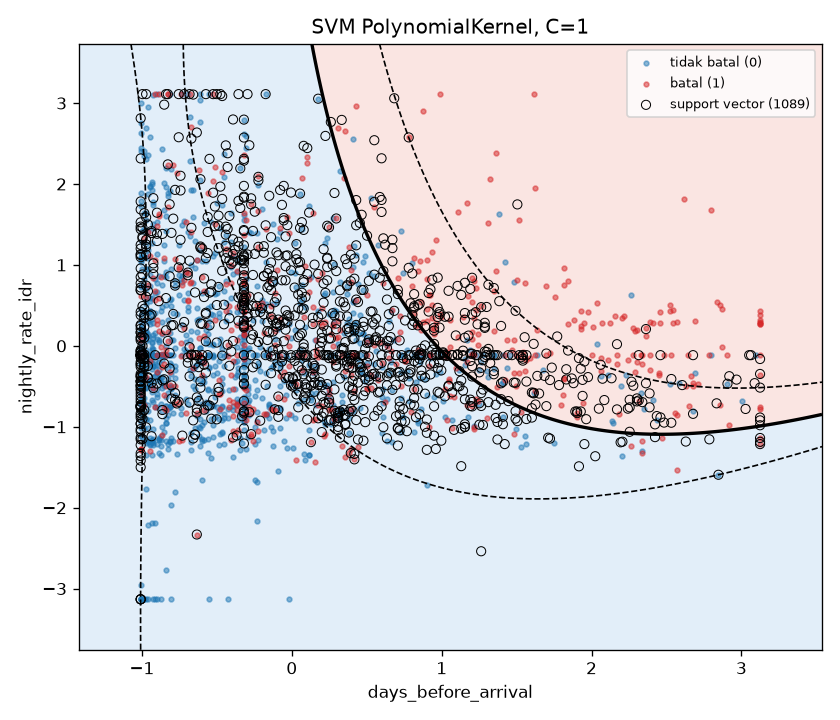
\includegraphics[width=0.32\textwidth]{output/svm_boundary_polynomial.png}\hfill
    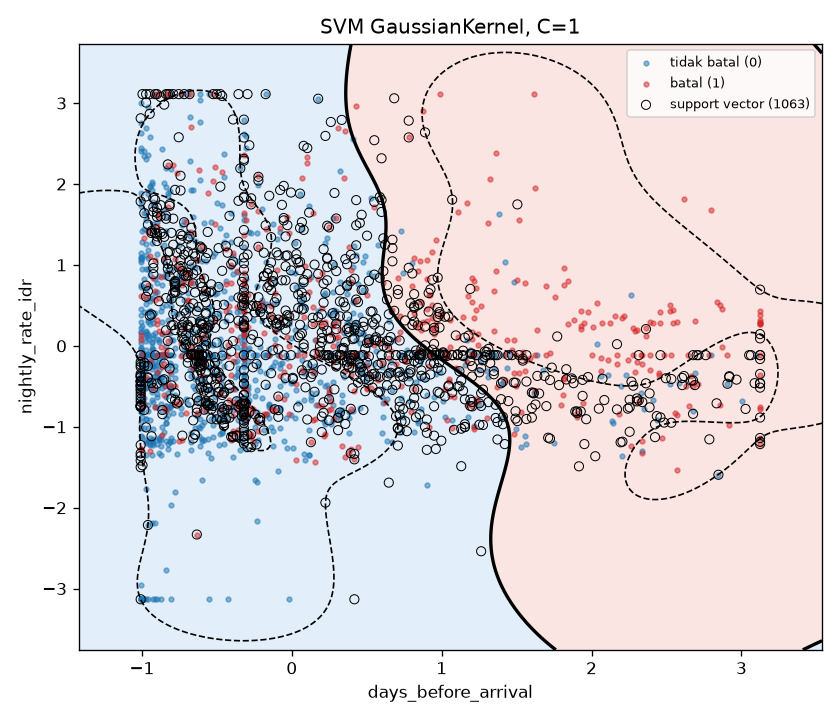
\includegraphics[width=0.32\textwidth]{output/svm_boundary_gaussian.png}
    \caption{Bidang pemisah, margin, dan \textit{support vector} untuk kernel linear, polinomial, dan Gaussian.}
    \label{fig:svm-boundary}
\end{figure}

\subsection{Algoritma Optimasi Model}
\subsubsection{FISTA dan Adam pada \textit{Logistic Regression}}
Eksperimen ini membandingkan kecepatan konvergensi \textit{gradient descent} (GD) proksimal, FISTA, dan Adam pada konfigurasi regularisasi baku ($\alpha=0{,}01$, \texttt{l1\_ratio}=0,5). Setiap \textit{optimizer} dijalankan 1.000 \textit{epoch} dengan \textit{batch} penuh dan tanpa kriteria berhenti dini. Objektif referensi adalah objektif terkecil dari FISTA yang dijalankan 20.000 \textit{epoch}. Tabel~\ref{tab:optim-lr} mencatat \textit{epoch} pertama saat objektif berada dalam $10^{-3}$ dan $10^{-4}$ dari referensi. Adam hanya diuji pada penalti L2 karena implementasinya terbatas pada fungsi tujuan yang mulus. Ukuran langkah FISTA $1/L$ bernilai sekitar 1,03 untuk kedua penalti.

\begin{table}[htbp]
    \centering
    \small
    \begin{tabular}{@{}l l r r r r r@{}}
        \toprule
        Penalti & \textit{Optimizer} & \multicolumn{2}{c}{\textit{Epoch} hingga} & Objektif akhir & Akurasi & Bobot nol \\
        \cmidrule(lr){3-4}
         & & $10^{-3}$ & $10^{-4}$ & & validasi & \\
        \midrule
        \multirow{3}{*}{Elastic Net} & GD, $\eta=0{,}1$ & 301 & 539 & 0,464751 & 0,7978 & 18 \\
         & GD, $\eta=0{,}5$ & 59 & 107 & 0,464746 & 0,7980 & 19 \\
         & FISTA, $\eta=1/L$ & \textbf{10} & \textbf{20} & 0,464746 & 0,7980 & 19 \\
        \midrule
        \multirow{4}{*}{L2} & GD, $\eta=0{,}1$ & 297 & 542 & 0,450102 & 0,7965 & 0 \\
         & GD, $\eta=0{,}5$ & 59 & 107 & 0,450093 & 0,7969 & 0 \\
         & FISTA, $\eta=1/L$ & \textbf{9} & \textbf{20} & 0,450093 & 0,7969 & 0 \\
         & Adam, $\eta=0{,}05$ & 27 & 67 & 0,450093 & 0,7969 & 0 \\
        \bottomrule
    \end{tabular}
    \caption{Kecepatan konvergensi GD, FISTA, dan Adam pada \textit{logistic regression} (1.000 \textit{epoch}).}
    \label{tab:optim-lr}
\end{table}

Semua \textit{optimizer} mencapai objektif yang sama hingga enam desimal, kecuali GD dengan laju baku 0,1 yang masih tertinggal sekitar $5\times10^{-6}$ setelah 1.000 \textit{epoch}. Akurasi validasi dan jumlah bobot nol juga sama, sehingga FISTA dan Adam tidak mengubah solusi, melainkan mempercepat jalan menuju solusi tersebut. FISTA paling cepat. FISTA membutuhkan 10 \textit{epoch} untuk mencapai jarak $10^{-3}$ pada Elastic Net, yaitu 30 kali lebih cepat daripada GD dengan laju baku dan hampir 6 kali lebih cepat daripada GD dengan laju 0,5 yang telah disetel. Keunggulan ini tidak memerlukan penyetelan laju belajar, karena $1/L$ dihitung langsung dari data. Adam pada penalti L2 membutuhkan 27 \textit{epoch}, sekitar dua kali lebih cepat daripada GD yang disetel, tetapi masih tiga kali lebih lambat daripada FISTA. Pada \textit{batch} penuh, momentum Nesterov dengan ukuran langkah yang tepat lebih efektif daripada laju belajar adaptif per parameter.

\subsubsection{\textit{Cost-Complexity Pruning} pada DTL}
\texttt{PrunedDecisionTree} pada \path{src/dtl_tuning.py} memangkas pohon C4.5 yang telah dilatih menggunakan kriteria Persamaan~\ref{eq:ccp}. Fungsi \texttt{prune\_node} bekerja dari daun ke akar. Subpohon diganti daun apabila galat kelas mayoritas sebagai daun ditambah $\alpha$ tidak melebihi jumlah biaya daun-daun subpohon tersebut. Kelas ini juga dapat memilih $k$ fitur teratas menurut \textit{mutual information} yang dihitung dari tabel peluang \textit{Naive Bayes} pada data latih lipatan.

\begin{lstlisting}[emph={prune_node},caption={Pemangkasan \textit{cost-complexity} (\texttt{src/dtl\_tuning.py})},label={lst:prune}]
def prune_node(node, alpha, total):
    counts = node.class_counts
    leaf_cost = min(counts[0], counts[1]) / total + alpha
    if node.is_leaf():
        return leaf_cost, node
    children, subtree_cost = {}, 0.0
    for key, child in node.children.items():
        cost, new_child = prune_node(child, alpha, total)
        children[key] = new_child
        subtree_cost += cost
    if leaf_cost <= subtree_cost:
        return leaf_cost, TreeNode(counts, node.n_samples, node.depth)
    return subtree_cost, replace(node, children=children)
\end{lstlisting}

Tabel~\ref{tab:prune} menyajikan validasi silang lima lipatan untuk dua konfigurasi: pohon baku dengan fitur turunan, serta konfigurasi \texttt{BEST} pada kode, yaitu fitur asli, 14 fitur teratas, dan \texttt{min\_gain}=$10^{-4}$. Pemangkasan ringan dengan $\alpha=5\times10^{-5}$ menaikkan akurasi kedua konfigurasi sekitar 0,35--0,4 poin persentase. Nilai $\alpha$ yang lebih besar menurunkan kinerja dengan cepat, karena pohon kehilangan aturan yang masih berguna. Konfigurasi \texttt{BEST} dengan $\alpha=5\times10^{-5}$ mencapai akurasi validasi silang 0,8506. Pada pembagian validasi utama, konfigurasi ini memperoleh akurasi 0,8552, F1 0,7639, dan ROC-AUC 0,9101, naik 1,0 poin persentase dari pohon C4.5 tanpa pemangkasan. Ukuran pohon menyusut dari 5.033 menjadi 820 simpul, sehingga model juga jauh lebih mudah ditafsirkan. Kenaikan ini muncul karena cabang-cabang dalam yang hanya mengikuti derau digantikan daun dengan distribusi kelas yang lebih stabil. CSV \path{output/submission_dtl_tuned.csv} dapat direproduksi persis dari konfigurasi ini.

\begin{table}[htbp]
    \centering
    \small
    \begin{tabular}{@{}l r r r r r@{}}
        \toprule
        Konfigurasi & $\alpha$ & Akurasi & F1 & ROC-AUC & Std. akurasi \\
        \midrule
        Baku (fitur turunan, semua fitur) & 0 & 0,8461 & 0,7542 & 0,8971 & 0,0041 \\
         & $2\times10^{-5}$ & 0,8480 & 0,7556 & 0,8989 & 0,0033 \\
         & $5\times10^{-5}$ & 0,8496 & 0,7549 & 0,9054 & 0,0042 \\
         & $10^{-4}$ & 0,8487 & 0,7504 & 0,8945 & 0,0044 \\
         & $10^{-3}$ & 0,8196 & 0,6983 & 0,8351 & 0,0049 \\
        \midrule
        \texttt{BEST} (fitur asli, 14 fitur) & 0 & 0,8467 & 0,7554 & 0,8968 & 0,0010 \\
         & $2\times10^{-5}$ & 0,8486 & 0,7564 & 0,8983 & 0,0005 \\
         & $5\times10^{-5}$ & \textbf{0,8506} & \textbf{0,7569} & \textbf{0,9065} & 0,0031 \\
         & $10^{-4}$ & 0,8494 & 0,7520 & 0,8996 & 0,0029 \\
         & $10^{-3}$ & 0,8193 & 0,6985 & 0,8293 & 0,0055 \\
        \bottomrule
    \end{tabular}
    \caption{Validasi silang lima lipatan DTL dengan berbagai nilai $\alpha$ pemangkasan.}
    \label{tab:prune}
\end{table}

\subsubsection{\textit{Random Search} dan Pembobotan Kolom pada KNN}
KNN baku memberi bobot yang sama kepada setiap kolom, sehingga kolom yang hampir tidak informatif ikut menentukan jarak. \texttt{WeightedKNN} pada \path{src/knn_tuning.py} mengalikan setiap kolom dengan bobot $w_j=(I_j/I_{\max})^{\gamma}$, dengan $I_j$ \textit{mutual information} kolom $j$ terhadap target yang dihitung dari data latih lipatan. Pada jarak Minkowski orde $p$, mengalikan kolom dengan $w_j$ setara dengan memberi bobot $w_j^{\,p}$ pada selisih kolom tersebut. Kelas ini juga dapat membuang kolom di luar \texttt{top\_k} teratas dan mengecilkan bobot kolom \textit{one-hot}. Model tetap berupa satu KNN, bukan \textit{ensemble}.

\begin{lstlisting}[emph={column_scale},caption={Bobot kolom berbasis \textit{mutual information} (\texttt{src/knn\_tuning.py})},label={lst:knn-weight}]
def column_scale(mi, names, gamma=0.0, top_k=0, onehot_factor=1.0):
    weight = np.ones(len(mi)) if gamma == 0 or mi.max() <= 0 else (mi / mi.max()) ** gamma
    if top_k:
        keep = np.zeros(len(mi))
        keep[np.argsort(-mi, kind="stable")[:top_k]] = 1
        weight = weight * keep
    onehot = np.array(["=" in str(n) for n in names])
    return np.where(onehot, weight * onehot_factor, weight)
\end{lstlisting}

Ruang pencarian mencakup jenis \textit{scaler}, pengodean siklik bulan ($\sin$ dan $\cos$), transformasi log untuk fitur miring, metrik jarak, $\gamma$, \texttt{top\_k}, faktor \textit{one-hot}, $k$, dan pembobotan tetangga. Ruang ini terlalu besar untuk \textit{grid search}, sehingga digunakan \textit{random search}. Pencarian memakai konfigurasi baku ditambah 30 konfigurasi acak dengan \texttt{seed=42}, dan setiap konfigurasi dievaluasi pada sembilan nilai $k$ dan dua pembobotan dengan validasi silang lima lipatan. Total terdapat 558 kombinasi. Seluruh langkah yang belajar dari data, termasuk \textit{mutual information}, di-\textit{fit} ulang di dalam setiap lipatan.

\begin{table}[htbp]
    \centering
    \small
    \setlength{\tabcolsep}{4pt}
    \begin{tabularx}{\textwidth}{@{}X r r r r r@{}}
        \toprule
        Konfigurasi & Akurasi CV & Std. & F1 CV & ROC-AUC CV & Akurasi validasi \\
        \midrule
        KNN baku (standar, Manhattan, $k=15$, \textit{distance}) & 0,8429 & 0,0016 & 0,7484 & 0,9049 & 0,8489 \\
        Terbaik: min-max, bulan siklik, Manhattan, $\gamma=0{,}5$, \texttt{top\_k}=24, $k=15$, \textit{distance} & \textbf{0,8612} & 0,0044 & \textbf{0,7809} & \textbf{0,9229} & \textbf{0,8639} \\
        \bottomrule
    \end{tabularx}
    \caption{Hasil \textit{random search} KNN dengan validasi silang lima lipatan.}
    \label{tab:knn-tune}
\end{table}

Tabel~\ref{tab:knn-tune} menunjukkan bahwa konfigurasi terbaik menaikkan akurasi validasi silang dari 0,8429 menjadi 0,8612 dan F1 dari 0,7484 menjadi 0,7809. Pada pembagian validasi utama, akurasinya 0,8639, sehingga KNN berbobot kolom lebih baik daripada seluruh konfigurasi sebelumnya. Enam konfigurasi teratas sama-sama memakai \textit{scaler} min-max, jarak Manhattan, $\gamma=0{,}5$, dan 24 kolom teratas. Pola ini menunjukkan bahwa sumber kenaikan terutama adalah pengurangan pengaruh kolom lemah pada jarak, bukan nilai $k$. \textit{Scaler} min-max juga membatasi setiap fitur pada rentang $[0,1]$, sehingga kolom \textit{one-hot} dan kolom numerik memiliki skala yang setara. Pencarian ini dijalankan ulang saat penyusunan laporan. CSV yang dihasilkan sama dengan \path{output/submission_knn_tuned.csv} pada 93,9\% baris, sehingga berkas tersebut kemungkinan berasal dari putaran pencarian yang berbeda.

\subsubsection{Penalti MDL pada Atribut Numerik DTL}
\texttt{MDLDecisionTree} pada \path{src/dtl_tuning.py} menurunkan kelas \texttt{DecisionTree} dan hanya mengganti pencarian ambang numerik. \textit{Gain} setiap kandidat ambang dikurangi $\log_2(N-1)/|D|$ seperti pada dasar teori, dengan $N-1$ jumlah kandidat ambang dan $|D|$ bobot sampel yang nilainya diketahui. Ambang dipilih berdasarkan \textit{gain} yang belum dipenalti, sedangkan nilai terpenalti dipakai untuk membandingkan antaratribut. Dengan cara ini, atribut numerik dengan banyak nilai unik, seperti tarif dan \texttt{days\_before\_arrival}, tidak lagi diuntungkan secara semu dibanding atribut kategorikal.

\begin{lstlisting}[caption={Penalti MDL pada \textit{gain} ambang numerik (\texttt{src/dtl\_tuning.py}, diringkas)},label={lst:mdl}]
penalised = gain - np.log2(len(positions)) / known_w
ratios = np.divide(penalised, split_info, out=np.zeros_like(gain), where=split_info > 1e-12)
valid &= (penalised > self.min_gain) & (split_info > 1e-12)
score = gain if self.threshold_by == "gain" else ratios
best = int(np.argmax(np.where(valid, score, -np.inf)))
\end{lstlisting}

Konfigurasi terbaik memakai penalti MDL, 14 fitur teratas, \texttt{min\_gain}=$10^{-4}$, pemangkasan $\alpha=5\times10^{-5}$, serta imputasi median dan modus sebagai pengganti bobot pecahan untuk nilai hilang. Tabel~\ref{tab:mdl} menunjukkan bahwa penalti MDL saja menaikkan akurasi validasi silang dari 0,8506 menjadi 0,8530. Penambahan imputasi menaikkan akurasi lagi menjadi 0,8585 dengan simpangan baku 0,0040. Pada data ini, imputasi tampaknya membantu karena bobot pecahan menyebarkan sampel bernilai hilang ke banyak daun kecil, sedangkan imputasi mengirim sampel tersebut ke satu cabang. Ambang keputusan 0,55 pada kode memberi akurasi validasi silang yang sama dengan ambang 0,5.

\begin{table}[htbp]
    \centering
    \small
    \setlength{\tabcolsep}{4pt}
    \begin{tabularx}{\textwidth}{@{}X r r r r r@{}}
        \toprule
        Konfigurasi DTL & Akurasi CV & Std. & F1 CV & ROC-AUC CV & Akurasi validasi \\
        \midrule
        Terpangkas tanpa MDL (\texttt{BEST}) & 0,8506 & 0,0031 & 0,7569 & 0,9065 & 0,8552 \\
        Terpangkas dengan MDL, bobot pecahan & 0,8530 & 0,0052 & 0,7622 & 0,9085 & 0,8566 \\
        Terpangkas dengan MDL dan imputasi & \textbf{0,8585} & 0,0040 & \textbf{0,7732} & 0,9010 & \textbf{0,8636} \\
        \bottomrule
    \end{tabularx}
    \caption{Pengaruh penalti MDL dan imputasi pada DTL terpangkas (ambang 0,5).}
    \label{tab:mdl}
\end{table}

Pohon akhir berisi 823 simpul. CSV \path{output/submission_dtl_mdl.csv} dapat direproduksi persis dari konfigurasi ini dengan ambang 0,55.

\subsubsection{Pipeline Kombinasi pada KNN}
Eksperimen terakhir pada KNN menggabungkan beberapa temuan sebelumnya ke dalam satu pipeline. \texttt{combo\_pipeline} tidak memakai fitur turunan dan tidak memotong pencilan, mengubah bulan kedatangan menjadi pasangan $\sin$ dan $\cos$, serta memperlakukan nilai hilang pada fitur kategorikal sebagai kategori tersendiri bernama \texttt{Missing}. Perlakuan terakhir ini dipilih karena hilangnya nilai kategori dapat membawa informasi sendiri, sebagaimana terlihat pada \texttt{special\_requests}. Model yang dipakai adalah \texttt{WeightedKNN} dengan $k=15$, jarak Manhattan, bobot jarak, $\gamma=0{,}5$, dan 20 kolom teratas.

\begin{lstlisting}[caption={Pipeline kombinasi KNN (\texttt{src/knn\_tuning.py})},label={lst:knn-combo}]
COMBO = {"k": 15, "metric": "manhattan", "p": 1, "weights": "distance", "gamma": 0.5, "top_k": 20}

def missing_as_category(df, cols=("meal_package", "room_category", "booking_channel")):
    df = df.copy()
    for c in cols:
        df[c] = df[c].fillna("Missing")
    return df

def combo_pipeline():
    return PreparationPipeline([cyclic_month, missing_as_category, Imputer(),
                                CategoricalEncoder(), Scaler("standard")])
\end{lstlisting}

Konfigurasi ini mencapai akurasi validasi silang 0,8651 dengan simpangan baku 0,0050, F1 0,7864, dan ROC-AUC 0,9267. Pada pembagian validasi utama, akurasinya 0,8674, F1 0,7928, dan ROC-AUC 0,9304. Dengan hasil tersebut, KNN dengan pipeline kombinasi menjadi model tunggal terbaik pada laporan ini, sedikit di atas KNN hasil \textit{random search} (0,8612) dan DTL dengan penalti MDL (0,8585). CSV \path{output/submission_knn_combo.csv} dapat direproduksi persis dari konfigurasi ini.

\subsubsection{Diskretisasi MDL pada \textit{Naive Bayes}}
Eksperimen ini mengganti 20 interval kuantil dengan ambang Fayyad--Irani, sementara fitur, $\alpha=1$, dan perlakuan nilai hilang tetap sama. Tabel~\ref{tab:nb-mdl} membandingkan kedua cara diskretisasi dengan validasi silang lima lipatan dan pada pembagian validasi utama.

\begin{table}[htbp]
    \centering
    \small
    \begin{tabular}{@{}l l r r r r r@{}}
        \toprule
        Diskretisasi & Evaluasi & Akurasi & Presisi & \textit{Recall} & F1 & ROC-AUC \\
        \midrule
        Kuantil, 20 interval & 5 lipatan & \textbf{0,7812} & \textbf{0,6871} & 0,6099 & 0,6462 & 0,8347 \\
        MDL Fayyad--Irani & 5 lipatan & 0,7800 & 0,6822 & \textbf{0,6149} & \textbf{0,6468} & 0,8347 \\
        \midrule
        Kuantil, 20 interval & validasi & 0,7784 & 0,6788 & 0,6148 & 0,6452 & 0,8364 \\
        MDL Fayyad--Irani & validasi & \textbf{0,7808} & 0,6787 & \textbf{0,6288} & \textbf{0,6528} & \textbf{0,8379} \\
        \bottomrule
    \end{tabular}
    \caption{Perbandingan diskretisasi kuantil dan MDL pada \textit{Naive Bayes}.}
    \label{tab:nb-mdl}
\end{table}

Kedua cara memberi kinerja yang hampir sama. Pada validasi silang, selisih akurasi hanya 0,0012 dan ROC-AUC sama hingga empat desimal, sedangkan pada pembagian validasi utama MDL sedikit lebih baik. Selisih sekecil ini masih berada dalam variasi antarlipatan, karena akurasi per lipatan berkisar 0,775 hingga 0,787. Perbedaan yang lebih jelas terlihat pada jumlah interval. MDL hanya memakai 8 ambang untuk \texttt{days\_before\_arrival} dan \texttt{nightly\_rate\_idr}, 5 ambang untuk \texttt{arrival\_month}, dan 3 ambang untuk \texttt{weekday\_nights}. \texttt{arrival\_day} tidak dipotong sama sekali, sehingga fitur ini praktis tidak berpengaruh pada posterior. Perubahan terpenting terjadi pada \texttt{prior\_completed\_bookings}. Batas kuantil fitur ini runtuh di nilai 0, sehingga seluruh 21.856 baris latih masuk ke satu interval dan \textit{mutual information}-nya nol. MDL menempatkan ambang di 0,5, yang memisahkan 477 tamu dengan riwayat pemesanan dari tamu lainnya, sehingga \textit{mutual information} fitur ini naik menjadi 0,0111 bit. Kelemahan yang dibahas pada Subbab~\ref{sec:hasil-nb} dengan demikian teratasi, tetapi sumbangannya kecil karena fitur tersebut hanya positif pada sekitar 2\% baris. Model dengan interval lebih sedikit ini lebih sederhana tanpa kehilangan kinerja, tetapi tidak menutup selisih terhadap pohon dan KNN. Batas utama \textit{Naive Bayes} tetap asumsi kebebasan bersyarat.

\subsubsection{Seleksi \textit{Working Set} Orde Kedua pada SMO}
\texttt{SVMWSS2} dilatih dengan kernel, $C$, subsampel 4.000 baris, dan toleransi yang sama dengan Tabel~\ref{tab:svm}. Tabel~\ref{tab:svm-wss} membandingkan jumlah iterasi SMO dan hasil validasinya.

\begin{table}[htbp]
    \centering
    \small
    \begin{tabular}{@{}l r r c r r r@{}}
        \toprule
        Kernel & \multicolumn{2}{c}{Iterasi SMO} & Konvergen & \multicolumn{2}{c}{Waktu \textit{fit} (detik)} & Tanda keputusan \\
        \cmidrule(lr){2-3}\cmidrule(lr){5-6}
         & Orde 1 & Orde 2 & (orde 2) & Orde 1 & Orde 2 & sama \\
        \midrule
        Linear & 100.000 & \textbf{54.788} & ya & 18,4 & \textbf{11,3} & 99,89\% \\
        Polinomial ($d=3$) & 60.733 & \textbf{9.842} & ya & 13,1 & \textbf{3,8} & 100\% \\
        Gaussian & 28.242 & \textbf{8.878} & ya & 6,2 & \textbf{3,4} & 100\% \\
        \bottomrule
    \end{tabular}
    \caption{Seleksi \textit{working set} orde pertama dan orde kedua pada SMO (subsampel 4.000 baris).}
    \label{tab:svm-wss}
\end{table}

Seleksi orde kedua mengurangi jumlah iterasi 3,2 kali pada kernel Gaussian dan 6,2 kali pada kernel polinomial. Pada kernel linear, versi orde pertama berhenti di batas 100.000 iterasi tanpa konvergen, sedangkan versi orde kedua konvergen pada 54.788 iterasi. Waktu \textit{fit} turun lebih sedikit daripada jumlah iterasi karena waktu tersebut juga mencakup perhitungan matriks kernel dan \textit{Platt scaling}. Akurasi, presisi, \textit{recall}, F1, dan ROC-AUC kedua versi sama hingga empat desimal pada ketiga kernel, dan tanda nilai keputusan pada data validasi sama pada sedikitnya 99,89\% baris. Hasil ini sesuai dengan rancangannya. Kriteria berhenti tidak berubah, sehingga kedua versi mencapai solusi dual yang sama dan perbedaannya hanya pada jalan menuju solusi. Penghematan waktu ini dapat dipakai untuk melatih SVM pada subsampel yang lebih besar.

\subsection{\textit{Submission} Kaggle}
Lima CSV dihasilkan dari konfigurasi pengumpulan, masing-masing satu per algoritma, dengan proporsi prediksi batal 24,6\% hingga 28,7\%. CSV DTL C4.5 dikirim ke Kaggle dan memperoleh skor publik 0,82005. Skor ini sekitar 2,5 poin persentase di bawah akurasi validasi lokal DTL (0,8451). Selisih tersebut dapat berasal dari variasi sampel pada leaderboard publik dan dari perbedaan metrik leaderboard, karena metrik yang dipakai Kaggle tidak diketahui secara pasti. Notebook pengumpulan bersifat \textit{reproducible} karena eksekusi ulang dari sel pertama menghasilkan \path{submission_decision_tree.csv} yang identik dengan berkas pada \path{output/}.
